\documentclass[12pt]{article}
\setlength\parindent{0pt}
\usepackage{fullpage}
\usepackage{color}
\usepackage[margin=0.5in]{geometry}
\usepackage{amsmath}
\usepackage{graphicx}
\setlength{\parskip}{1.5em}
\def\LL{\left\langle}   % left angle bracket
\def\RR{\right\rangle}  % right angle bracket
\def\LP{\left(}         % left parenthesis
\def\RP{\right)}        % right parenthesis
\def\LB{\left\{}        % left curly bracket
\def\RB{\right\}}       % right curly bracket
\def\PAR#1#2{ {{\partial #1}\over{\partial #2}} }
\def\PARTWO#1#2{ {{\partial^2 #1}\over{\partial #2}^2} }
\def\PARTWOMIX#1#2#3{ {{\partial^2 #1}\over{\partial #2 \partial #3}} }
\newcommand{\BI}{\begin{itemize}}
\newcommand{\EI}{\end{itemize}}
\newcommand{\BE}{\begin{displaymath}}
\newcommand{\EE}{\end{displaymath}}
\newcommand{\BNE}{\begin{equation}}
\newcommand{\ENE}{\end{equation}}
\newcommand{\BEA}{\begin{eqnarray}}
\newcommand{\EEA}{\nonumber\end{eqnarray}}
\newcommand{\EL}{\nonumber\\}
\newcommand{\la}[1]{\label{#1}}
\newcommand{\ie}{{\em i.e.\ }}
\newcommand{\eg}{{\em e.\,g.\ }}
\newcommand{\cf}{cf.\ }
\newcommand{\etc}{etc.\ }
\newcommand{\Tr}{{\rm tr}}
\newcommand{\etal}{{\it et al.}}
\newcommand{\OL}[1]{\overline{#1}\ } % overline
\newcommand{\OLL}[1]{\overline{\overline{#1}}\ } % double overline
\newcommand{\OON}{\frac{1}{N}} % "one over N"
\newcommand{\OOX}[1]{\frac{1}{#1}} % "one over X"



\begin{document}
\Large
\centerline{\sc{Recitation Exercises}}
\normalsize
\centerline{\sc{April 15}}

\pagenumbering{gobble}

\begin{enumerate}

\item {Formula One race cars use a ``kinetic energy recovery system'' that stores energy in rapidly spinning wheels, called flywheels. When the car slows down to make a turn, the car couples the flywheel to the transmission; it begins to spin rapidly, storing some of the car's translational kinetic energy in its rotation. One type of these systems uses a flywheel of mass $m=5$ kg and radius $r=12$ cm that rotates at up to 60,000 revolutions/minute.

You can model the flywheel as a uniform cylinder ($I=\frac{1}{2}mr^2$).


a) What is its angular velocity in radians per second?

{\color{red} Here we want them to get used to just converting these units and reminding them what $\omega$ means.}

{\color{blue} 60000 rpm = 1000 rev/sec = 6283 rad/sec.}

b) How much energy does it store when rotating at full speed?
{\color{red} Here they just plug into $$KE_{rot} = \frac{1}{2}I \omega^2.$$ They'll need to look up the moment of inertia in the attached table.}

{\color{blue}$$KE_{rot} = I \omega^2 = \frac{1}{2} \left(\frac{1}{2}mr^2\right) \omega^2 = 648\,\text{kJ}.$$ 

They should take care to not forget the second factor of 1/2 -- one comes from the formula for kinetic energy; one comes from $I=\frac{1}{2}mr^2$ for a cylinder. }


c) Suppose the wheel is only spinning at half speed (30,000 rpm). What fraction of its maximum energy does it store? \textit{(You should be able to answer this without a calculator. If you are not sure how, ask your instructors for advice.)}

{\color{red}  This is the first of many things we will do in recitation to try to reinforce their skills at proportional reasoning (that they failed at on the exam's spring problem). No calculators here!}

{\color{blue} The logic: energy is proportional to $\omega^2$ so if $\omega$ is half as big, energy is half squared = 1/4 as big.}



d) When the car accelerates again, this system uses the rotational energy stored in the flywheel to supplement the engine power. If the system provides 60 kW of extra power, how many seconds of ``boost power'' can the system deliver before it is out of energy?

{\color{red}  Here we are reminding them that power = energy per time, so time = energy over power.}

{\color{blue} $$648\, {\text {kJ}} / 60 \, \text{kW} = 10.8 \,\rm s$$

}

\newpage

\item {

As we did in class, consider rolling different objects down a slope of height $h$. In this exercise, you will determine how fast they are moving (their final speed $v$) when they reach the bottom.

First, consider a solid cylinder of mass $m$ and radius $r$. 

For each of the following, your group should guess whether it will be moving \textit{faster, slower, or the same speed} than the original cylinder when it reaches the bottom. You haven't done any calculations yet, so you may not know for sure -- that's okay! Record the result you expect and a brief reason why.

\begin{itemize}
\item A more massive solid cylinder of mass $2m$ with the same radius $r$
\item A larger solid cylinder with the same mass $m$, but with radius $2r$
\item A hollow cylinder, also of mass $m$ and radius $r$
\item A solid sphere, also of mass $m$ and radius $r$
\end{itemize}

{\color{red}  
Here we are okay with educated guesses. We did the demo but didn't do the calculation in full in either class -- so we didn't get to the result that the mass doesn't matter (which we might expect, since it generally cancels in things like this). We saw another problem where the radius cancels, but not this exact one, so they {\it might} be able to surmise that the radius doesn't matter either and that {\it only} the shape matters.

So: all the solid cylinders ($I=\frac{1}{2}m\omega^2$) are the same. All the hollow cylinders ($I = m \omega ^2$) are slower: one piece of logic they might use is that the mass is further to the outside, meaning that more energy goes into rotation with less available to produce translation. This is reflected by the higher number in front of the moment of inertia.

All the solid spheres are faster, since $I = \frac{2}{5} m \omega ^2$.

}

{\color{blue}
	
}


\vspace{0.4in}

Now, we'll calculate how fast each of them go down the slope. First, consider a hollow cylinder rolling down the slope. As it rolls, its potential energy at the top is converted into kinetic energy. You may write things in terms of $g$, $m$, $r$, $h$, etc. here; we don't have any numbers.



{\color{red}
Here we want them to do this particular problem, but also to see that the ideas of work and energy apply to motion including rotation as well. Clever students may ask about the force of friction between the rolling thing and the slope; it doesn't do any work, but we aren't fully equipped to see why yet since we need torque for that. The standard textbook explanation is that the point of contact of a rolling object is momentarily stationary so the displacement is zero so the work is zero, but I've always found that unsatisfying.
}



\begin{enumerate}
	\item What is its total energy at the top of the slope?
\vspace{0.7in}

{\color{blue}
	The potential energy at the top is of course
	
	$$PE = mgh.$$
}

    \item What is its total energy at the bottom of the slope? (Hint: What kinds of energy does it have there?)
    
    
    {\color{red}
    Here we want them to realize that a rolling object combines translation and rotation. {\it We did not have time to go over this as fully in class as I would like}, so you will need to talk to them about that. Short explanation:
    
    \begin{itemize}
    \item If an object rolls, then it is both turning and moving
    \item So we have both $\frac{1}{2}mv^2$ of translational kinetic energy, where $v$ is how fast it is moving, and $\frac{1}{2}I\omega^2$ of rotational kinetic energy
    \end{itemize}
    }
    {\color{blue}
    
    At the bottom, then, we have 
    
    $$E_{\rm{total}} = \frac{1}{2}mv^2 + \frac{1}{2}I \omega ^2.$$
    
    }
    
    \item If you set these two expressions for the total energy equal (since no other force does work here, and since energy is conserved), you will arrive at an equation that you could solve for $v$, the speed that the ball is moving at the bottom. However, it has another unknown in it: $\omega$, the rate at which it is rotating.
    
    However, the ball is rolling without slipping. What condition relates $v$ to $\omega$ if the ball rolls without slipping?
    
        {\color{red}
    Here they need the following logic: rolling without slipping is some combination of translation and rotation that keeps the point of contact stationary. So this means that as the object's translation carries it forward, its rotation (about its center) must make the point of contact move backwards relative to its center by the same amount. (``If you're driving at 50 miles per hour, your tires are also spinning at 50 miles per hour.'')
    
    This leads them to
    
    $$v = \omega r.$$
    	
    }
    
    
    
    \vspace{1in}
    \newpage
    
    \item Make this substitution, and arrive at an expression for $v$. What does it depend on? What does it not depend on?
    
          {\color{red}
    The math pattern that appears here is {\bf very common} and important for them to recognize. Here the $r^2$ that comes from the moment of inertia will cancel with the $r^2$ that comes from $\omega^2 = v^2/r^2$. There are two common ways to see this.
    }
    
    {\color{blue} Method 1:
    	
    	$$mgh = \frac{1}{2}mv^2 + \frac{1}{2}I \omega ^2$$
    	
    	Substitute in for $I$:
    	
    	$$mgh = \frac{1}{2}mv^2 + \frac{1}{2} \left(mr^2\right) \omega ^2$$
    	
    	Regroup this to make it obvious what we're about to do:
    	
    	$$mgh = \frac{1}{2}mv^2 + \frac{1}{2} m\left(r^2 \omega ^2\right)$$
    	
    	Now we observe that $r^2 \omega^2 = v^2$:
    	
    	$$mgh = \frac{1}{2}mv^2 + \frac{1}{2} mv^2$$
    	
    	$$mgh = mv^2 \rightarrow v = \sqrt{gh}$$
    	
    	Method 2: the other approach involves determining that $\omega = v/r$ and substituting that in:
    	
    	$$mgh = \frac{1}{2}mv^2 + \frac{1}{2}I \omega ^2$$
    	
    	Substitute in for $\omega = v/r$ and $I$:  	
    	$$mgh = \frac{1}{2}mv^2 + \frac{1}{2} \left(mr^2\right) \frac{v^2}{r^2}$$
    	
    	Now we cancel the $r$'s and get the same answer as before:
      	
    	$$mgh = \frac{1}{2}mv^2 + \frac{1}{2} mv^2$$
    	
    	$$mgh = mv^2 \rightarrow v = \sqrt{gh}$$
    	
    }

    Now, we'll consider objects other than a hollow cylinder: a solid ball, a solid cylinder, and a hollow ball. These will have different forms for the moment of inertia: instead of $I=mr^2$, their moments of inertia have the form $I=\lambda mr^2$, where $\lambda$ is a fraction. 
    
    We could do these calculations one at a time, but it is much faster to do the calculation leaving $\lambda$ in the expression for $I$; then you can substitute in at the end.
    
    Repeat the above calculation for all of these other shapes. You'll arrive at a general formula for the speed of an object (whatever its shape) of mass $m$ and radius $r$ after rolling down a hill of height $h$.
    
      {\color{red}
  	This is {\bf not scary} but they may think it is. If they're afraid, have them look at the moment of inertia chart and realize that it's always some fraction times $mr^2$. I use the symbol $\lambda$ for that fraction but that's arbitrary. So $\lambda$ = 1/2 for a cylinder, 2/3 for a hollow ball, etc.
  }
{  \color{blue}
    	
    $$mgh = \frac{1}{2}mv^2 + \frac{1}{2} \lambda I \omega ^2$$
    
    Substitute in for $I$:
    
    $$mgh = \frac{1}{2}mv^2 + \frac{1}{2} \left(\lambda mr^2\right) \omega ^2$$
    
    Regroup this to make it obvious what we're about to do:
    
    $$mgh = \frac{1}{2}mv^2 + \frac{1}{2} \lambda m\left(r^2 \omega ^2\right)$$
    
    Now we observe that $r^2 \omega^2 = v^2$:
    
    $$mgh = \frac{1}{2}mv^2 + \frac{1}{2} \lambda mv^2$$
    
    $$mgh = (1 + \lambda)mv^2 \rightarrow v = \sqrt{\frac{2gh}{1 + \lambda}}.$$
    
    Point out that this is generally true for any object of any shape -- you can use this one formula to understand cylinders, hollow balls, rings, whatever.
    
}
    \vfill Check your result with your TA once you have it.
    
    \newpage
    
    \item Here's our list of objects again.
    
\begin{itemize}
	\item A solid cylinder of mass $m$ and radius $r$
	\item A more massive solid cylinder of mass $2m$ with the same radius $r$
	\item A larger solid cylinder with the same mass $m$, but with radius $2r$
	\item A hollow cylinder, also of mass $m$ and radius $r$
	\item A solid sphere, also of mass $m$ and radius $r$
\end{itemize}
    
    Rank them in order of how quickly they'll be moving when they reach the bottom of the ramp. Think about which quantities ($m$, $r$, and the shape) appear in your formula and which don't.
    
\end{enumerate}
}
   {\color{red}
Challenge the students to go back over their math and think about why mass and radius don't matter. Mass doesn't matter because it appears in every term -- gravitational potential energy, and translational and rotational kinetic energy. The radius is harder -- the reason it doesn't matter is that an object with a larger radius has a  higher moment of inertia, but it also can rotate slower to satisfy $v = \omega r$, the rolling constraint. These factors are both squared, so they cancel.

Here they should realize that the only thing that matters is $\lambda$, and the things with the higher $\lambda$ go slower. So in order, from slowest to fastest: hollow cylinder ($\lambda=1$), all the solid cylinders ($\lambda = 1/2$), then the sphere ($\lambda = 2/5$)
}
\vspace{3in}

\item In the previous exercise, you arrived at a formula for $v_f$ in terms of $g$, $h$, and $\lambda$.

\bigskip\bigskip

Suppose that you have some other ramp. You observe that when you roll a hollow sphere down it, it's traveling at 1 m/s. How fast would a solid sphere be traveling? \textit{(You do have enough information to provide a number here, even though you don't know $m$, $g$, $h$, or $r$.)}
}

   {\color{red} This is another callback to the spring problem on the exam: comparing things by looking at how the formula changes when you change something. On the exam they couldn't deal with this since most don't read equations as ``statements about nature'', but only as ``stuff you plug stuff into'', so they had trouble with not knowing $m$ or $k$. Here they will have trouble not knowing $h$, $m$, $r$, etc.
   	
   	There are two ways to do this, the mathy way and the intuitive way.
   	
   	Intuitive way: the velocity is inversely proportional to $\sqrt{1+\lambda}$. So I should multiply by 
   	
   	$$\sqrt \frac{1+\lambda_{\rm old}}{1+\lambda_{\rm new}} = \sqrt \frac {1+2/3}{ 1+2/5} = 1.091$$
   	
   	which gives me 
   	
   	$$v = 1.091 \, \rm m/\rm s.$$
   	
   	More mathy way:
   	
   	Use the formula from before twice, for the hollow sphere (object 1) and the solid one (object 2):

   	$$v_1 = \sqrt{\frac{2gh}{1 + \lambda_1}}$$
   	
	$$v_2 = \sqrt{\frac{2gh}{1 + \lambda_2}}$$
	
	Divide one of these by the other, deal with the grossness that happens when you use brute force rather than intuition, and cancel stuff:
	
		$$\frac{v_2}{v_1} = \frac{\sqrt{\frac{2gh}{1 + \lambda_2}}}{\sqrt{\frac{2gh}{1 + \lambda_1}}} =\sqrt \frac{{\frac{2gh}{1 + \lambda_2}}}{{\frac{2gh}{1 + \lambda_1}}} = \sqrt \frac{1+\lambda_{\rm 1}}{1+\lambda_{\rm 2}}$$
			
	Then
	
	$$v_2 = v_1 \sqrt \frac{1+\lambda_{\rm 1}}{1+\lambda_{\rm 2}} = 1.091 \, \rm m/\rm s.$$

   	
}

\end{enumerate}

\newpage


\begin{center}
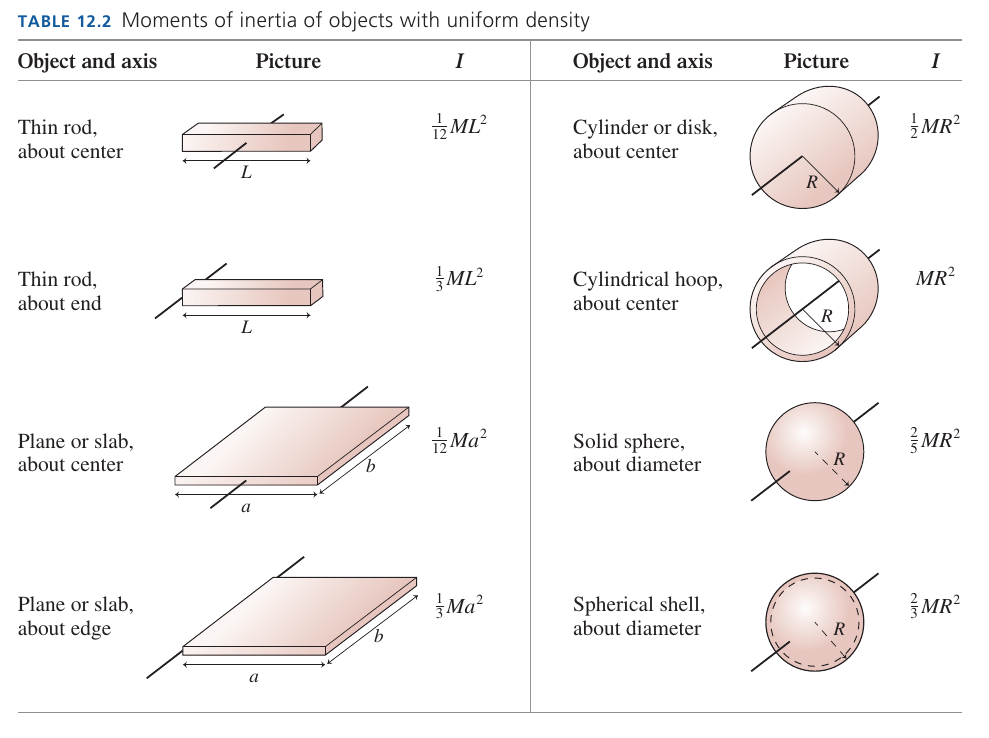
\includegraphics[width=7in]{moment-table.png}
\end{center}

\end{document}
